\chapter{Detalji implementacije}
\label{ch:implementacija}

U ovoj glavi opisani su izvršeni eksperimenti, kao i struktura koda. Implementacija i testiranje zasnovani su na radovima \cite{dqn_mnih} i \cite{dqn_dm}.
\section{Detalji implementacije}
\label{sec:implementacija}
Prilikom implementacije, korišćen je programski jezik Python \cite{python}, verzija $3.5.2$ kao i sledeće biblioteke:
\begin{itemize}
	\item \texttt{NumPy} \cite{numpy} -- Biblioteka otvorenog koda za numeričko izračunavanje. Korišćena je verzija $1.14.1$.
	%	1.14.1
	% http://www.numpy.org/ 
	\item \texttt{Keras} \cite{keras} -- Biblioteka otvorenog koda koja pruža visoko apstraktni API, što je čini jednostavnim za korišćenje. Ova biblioteka zahteva pozadinsku biblioteku za izračunavanje; u ovu svrhu je korišćena biblioteka \texttt{TensorFlow}\cite{tensorflow}. Verzija biblioteke \texttt{Keras} koja je upotrebljavana je $2.2.0$, dok je verzija biblioteke \texttt{TensorFlow} $1.5.0$.
	%	2.2.0
	% https://keras.io/
	\item  \texttt{OpenAI~Gym} \cite{openai_gym} -- Biblioteka otvorenog koda koja pruža mogućnost korišćenja već gotovih okruženja radi istraživanja raznih pristupa učenju potkrepljivanjem. Korišćena je verzija $0.10.5$ ove biblioteke.
	%	0.10.5
	% https://gym.openai.com/
\end{itemize}
% PYTHON: 3.5.2
% KERAS: 2.2.0
% OPENAI GYM: 0.10.5
% TENSORFLOW: 1.5.0
% NUMPY: 1.14.1
Implicitno su korišćene i biblioteke od kojih navedene biblioteke zavise. U sklopu implementacije korišćeni su i neki moduli koji su deo standardne biblioteke jezika python.
\par 
Implementacija $DQN$ sastoji se iz dve klase, {\em DQNAgent} i {\em ExperienceReplay}, i nekoliko pomoćnih funkcija. Struktura koda opisana je u nastavku, na apstraktnom nivou. Ovo znači da su opisi nekih funkcija, koje nisu od važnosti za shvatanje koda, izostavljeni. Izvorni kod može se naći na sledećoj adresi: \url{https://github.com/NikolaMilev/DQN}.
\par 
Klasa \texttt{DQNgent} opisuje funkcionisanje agenta koji se obučava prateći $DQN$ algoritam. Glavne komponente klase su memorija i dve neuronske mreže: Q mreža i ciljna mreža.

Glavne komponente klase su memorija i $Q$ i ciljna mreža. Metodi bitni za učenje su:
\begin{itemize}
	\item \texttt{chooseAction(self, state)}\footnote{Pri pisanju instancnih metoda u jeziku python, prvi argument je uvek referenca na objekat nad kojim se taj metod poziva. Ta referenca označava se ključnom reči \texttt{self}} -- Vrši odabir akcije na osnovu stanja koje je prosleđeno referencom \texttt{state}. Odabir se vrši u skladu sa $\varepsilon$-pohlepnom politikom.
	\item \texttt{trainOnBatch(self, batchSize)} -- Trenira $Q$ mrežu nasumičnim uzorkovanjem memorije, koristeći formule opisane u algoritmu \ref{alg:dqn}.
	\item \texttt{test(self, network, numSteps)}\footnote{Parametar \texttt{network} stoji jer je isti kod korišćen za obučavanje raznih varijacija algoritma pri ispitivanju njegovih komponenti.} -- Vrši testiranje mreže date argumentom \texttt{network} u skladu sa pravilima opisanim u delu \ref{sec:testiranje}. Testiranje traje \texttt{numSteps} koraka.
	\item \texttt{learn(self)} -- Vrši obučavanje agenta. 
\end{itemize}
\par 
Klasa \texttt{ExperienceReplay} opisuje omotač oko klase \texttt{deque}, koja opisuje objedinjenje pojmova steka i reda.\footnote{Dokumentacija ove klase može se naći na adresi \url{https://docs.python.org/3/library/collections.html\#collections.deque}.} Bitni metodi klase su:
\begin{itemize}
	\item \texttt{addTuple(self, state, action, reward, nextState, terminal)} -- Dodaje petorku \texttt{(state, action, reward, nextState, terminal)} u memoriju. Prva četiri elementa odgovaraju četvorki $(s, a, r, s')$, odnosno jednom prelazu koji je agent video, dok peti element predstavlja istinitosnu vrednost koja označava da li je stanje $s'$ završno. Ovu informaciju neophodno je čuvati jer se ona ne nalazi u samim stanjima.
	\item \texttt{getMiniBatch(self, sampleSize)} -- Dohvata uzorak veličine \texttt{sampleSize} iz memorije.
\end{itemize}
\par 
Pored opisanih klasa, kod sadrži i funkcije koje pomažu boljoj strukturi koda:
\begin{itemize}
	\item \texttt{buildNetwork(height, width, depth, numActions)} -- Koristeći pozive iz biblioteke Keras, gradi neuronsku mrežu i vraća referencu na dati objekat.
	\item \texttt{copyModelWeights(srcModel, dstModel)} -- Kopira težine mreže \texttt{srcModel} u mrežu \texttt{dstModel}.
	\item \texttt{saveModelWeights(model, name)} -- Čuva neuronsku mrežu čija referenca se prosleđuje argumentom \texttt{model} na putanju određenu argumentom \texttt{name}.
	\item \texttt{preprocessSingleFrame(img)} -- Vrši pretprocesiranje jedne slike sa ekrana, opisano u \ref{sec:pretprocesiranje}.
	\item \texttt{transformReward(reward)} -- Transformiše nagradu.
\end{itemize}
\par 
U više navrata je rečeno da $DQN$ algoritam uči nad slikama ekrana i nagradom dobijenom od okruženja. Međutim, jedna slika ne daje mnogo informacija. Na primeru igre Breakout, ukoliko je dostupna samo jedna slika ekrana, nemoguće je odrediti u kom se pravcu kreće loptica, ni kojom brzinom. Isto važi i za pločicu koja služi za odbijanje loptice. Međutim, iz nekoliko uzastopnih slika može se odrediti smer i brzina kretanja loptice i pločice. Na slici \ref{fig:ss} prikazane su četiri uzastopne slike sa ekrana.\footnote{Radi ilustracije, nisu prikazane uzastopne slike već je razlika između njih 7 slika. Prikazivanje uzastopnih slika sa ekrana dalo bi kao rezultat 4 skoro identične slike.} 

\begin{figure}
	\centering
	\resizebox{.24\linewidth}{!}{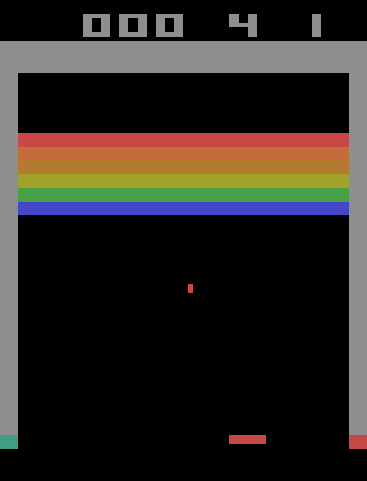
\includegraphics{img/screenshots/1}}
	\resizebox{.24\linewidth}{!}{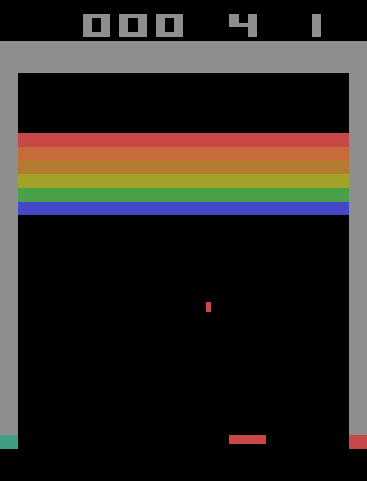
\includegraphics{img/screenshots/2}}
	\resizebox{.24\linewidth}{!}{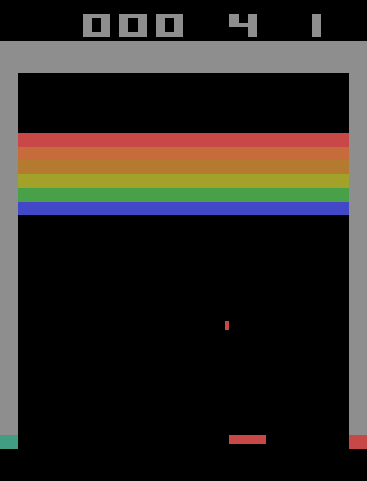
\includegraphics{img/screenshots/3}}
	\resizebox{.24\linewidth}{!}{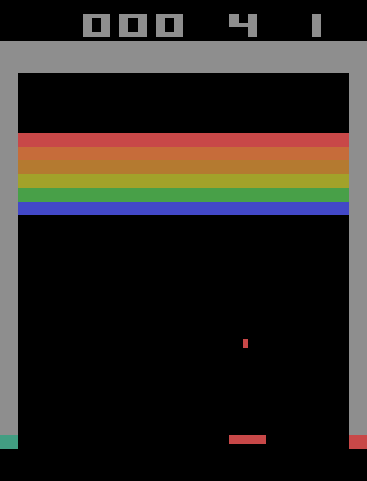
\includegraphics{img/screenshots/4}}
	\caption{Prikaz 4 uzastopna stanja ekrana u igri Breakout. Pločica miruje dok se loptica kreće ka donjem desnom uglu ekrana.}
	\label{fig:ss}
\end{figure}
\par 
Kako igre sa Atari 2600 konzole prikazuju $60$ slika u sekundi (eng.~{\em frame per second},~skr.~{\em fps}) i kako nije realno delati tom frekvencijom, vrši se preskakanje slika (eng.~{\em frame skipping}). Biblioteka \texttt{OpenAI Gym} pruža mogućnost korišćenja raznih vrednosti za broj preskočenih slika. U ovom radu, koristi se okruženje pod imenom \texttt{BreakoutDeterministic-v4},\footnote{Ovo okruženje ne može se naći u zvaničnoj dokumentaciji.} što znači da će okruženje za jedan poziv kojim se vrši akcija izvršiti tu akciju na $4$ uzastopne slike koja se prikazuje. Deo imena \texttt{Deterministic} označava da će se uvek pozivom prikazivati svako četvrto stanje ekrana; neka okruženja dopuštaju da se preskakanje vrši nasumično, u nekom intervalu dozvoljenih vrednosti. Na primer, okruženje \texttt{Breakout-v0} za svaki poziv vrši preskakanje nasumično odabranog broja slika iz intervala $[1,4]$. U ovoj implementaciji, po uzoru na rad \cite{dqn_dm}, agent će videti svako četvrto stanje ekrana. 
\par 
Na svake $4$ viđene slike, vršiće se jedan korak stohastičkog gradijentnog spusta, nasumičnim uzorkovanjem $32$ elementa memorije.

\subsection{Prelazi i čuvanje u memoriji}

U cilju čuvanja informacija o smeru kretanja objekata na ekranu, svako stanje biće sačinjeno od određenog broja uzastopnih slika koje agent vidi. Svaki prelaz sačuvan u memoriju u stvari je petorka oblika $(s, a, r, s', t)$. 
Ono na šta pri implementaciji treba obratiti pažnju su memorijski zahtevi. Nakon transformacije, dobijene slike su dimenzija $105 \times 80$ i njihove koordinate implicitno su zapisane u pokretnom zarezu. Ukoliko je jednostruka tačnost u pitanju, jedno stanje zauzima $32.8~kB$. Dakle, čuvanje milion stanja, kako je predloženo u radu \cite{dqn_dm}, zahteva između $32$ i $33~GB$ memorije. Ovo je moguće popraviti. Naime, kako su vrednosti dobijene nakon transformacije u intervalu $[0, 255]$ i kako će kasnije biti transformisane tako da staju u interval $[0, 1]$, to je bez gubitka značajne količine podataka moguće zaokružiti ih i čuvati ih u jednobajtnom podatku. Biblioteka \texttt{NumPy} definiše tip \texttt{uint8} koji ovo omogućuje. Takođe treba paziti na to da dva uzastopna stanja dele sve sem jedne slike. Ukoliko se stanja definišu tako da sadrže reference na pojedinačne slike umesto pravljenja novog niza, deljenje referenci osigurava da se neće praviti bespotrebne kopije podataka. Zajedno sa ostalim memorijskim zahtevima, prilikom treniranja agenta bilo je zauzeto oko {\em 10~GB} memorije.

